%!TEX root = ../thesis.tex
%*******************************************************************************
%****************************** Evaluation Chapter *********************************
%*******************************************************************************

\chapter{Evaluation}
\label{chap:evaluation}
In the previous chapter, we explained the implementation of our tool. 
Based on that, in this chapter, we will discuss the details of the evaluation process, including the user case study (see section \ref{evaluation:section:casestudy}), experimental design (see section \ref{evaluation:section:design}), execution (see section \ref{evaluation:section:execution}), analysis (see section \ref{evaluation:section:analysis}), and interpretation (see section \ref{evaluation:section:interpretation}) of the results. 
For the setup, we recruited participants from Paderborn University.
\ifpdf
    \graphicspath{{Chapters/Evaluation/Figs/}{Chapters/Evaluation/Figs/}{Chapters/Evaluation/Figs/}}
\else
    \graphicspath{{Chapters/Evaluation/Figs/}{Chapters/Evaluation/Figs/}}
\fi

\section{User Case Study}
\label{evaluation:section:casestudy}
To evaluate the effectiveness of our approach, we conducted a case study that involved recruiting participants, developing prototypes, and working on user scenarios. 
We recruited 15 participants who are students at Paderborn University. 
The case study is based on the evaluation stage of the first cycle of our DSR (as discussed in section \ref{introduction:section:research}). 
In conducting and reporting our case study research, we followed the established guidelines of Runeson and Höst \cite{eval:guidlines:runeson} (see figure \ref{evaluation:fig:casestudy}) to increase the quality of the study outcomes. 
These guidelines helped ensure our research was rigorous, transparent, and credible. 
By adhering to these guidelines, we aimed to provide a detailed and comprehensive account of our case study, enabling others to replicate our research and build upon our findings.
This case study also aims to develop the RQ as explained in the next section.

\clearpage
\section{Experimental Design}
\label{evaluation:section:design}
In this section, as per Runeson and Höst, we first define the objective, case study, research questions, and the methods we follow to complete the evaluation.

\paragraph{Objective:}
The objective of the user case study was to evaluate a \ac{poc} tool for creating and testing UI designs. 
The goal was to assess the tool's ability to generate UI prototypes, create split or A/B tests, and collect participant feedback to select the best variant.

\paragraph{Case Study:}
The case study involved a user scenario where John, a UX designer, was responsible for designing the UI for a new movie-streaming app. John used the \ac{poc} tool to create UI prototypes and perform split tests to select the best variant.

\paragraph{Research Questions (RQs):}
For the case study, we defined a couple of research questions. \\
\textbf{RQ1:} Can a \ac{poc} tool be used to prototype the UI of a new movie-streaming app and create split or A/B tests to select the best variant of the app's interface design? \\
\textbf{RQ2:} What feedback can be gathered from participants to evaluate the effectiveness of different app interface design variants?

\begin{figure}[ht]
    \centering
    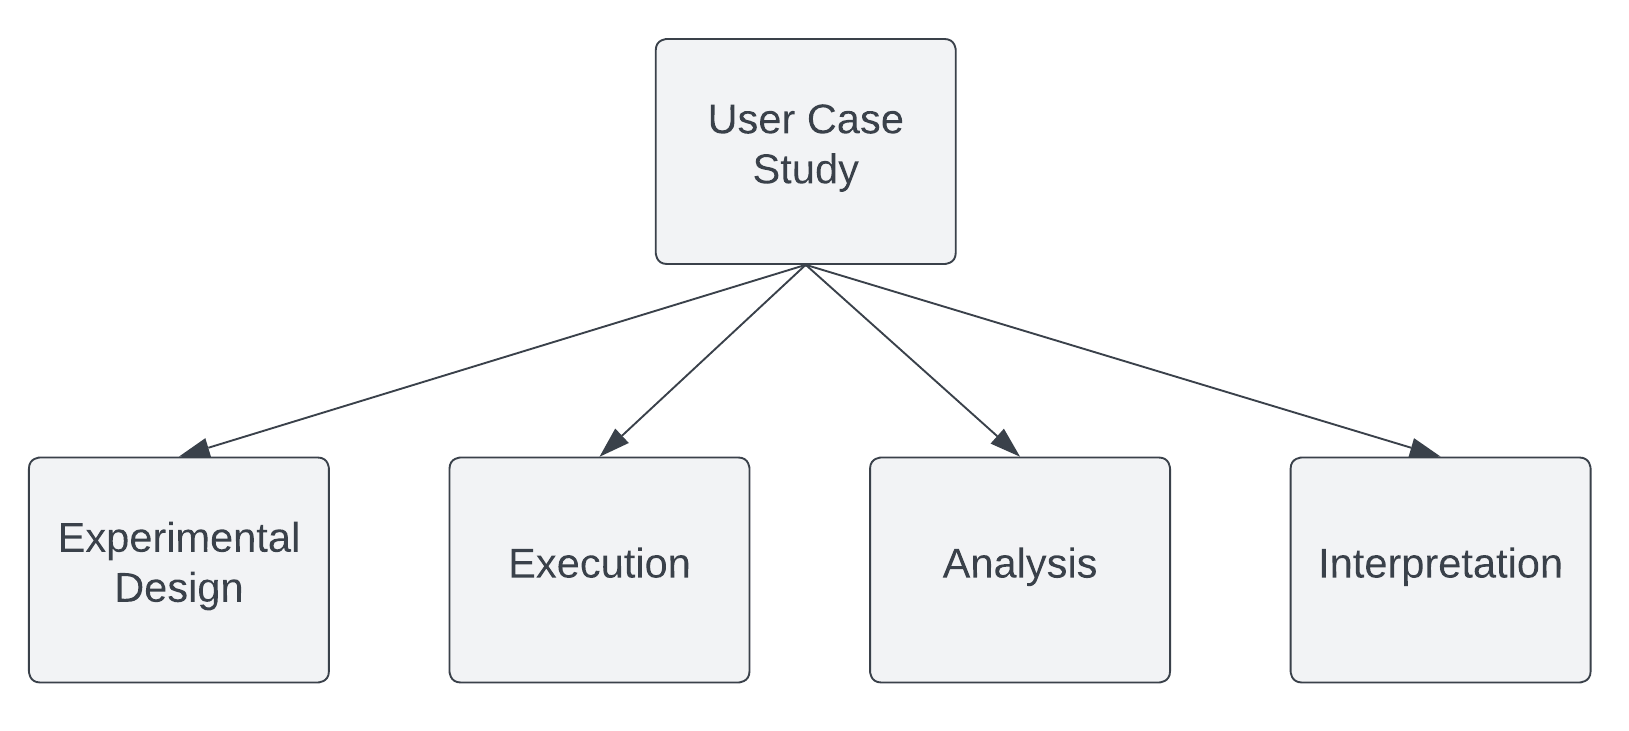
\includegraphics[scale=0.25]{case-study.png}
    \caption{User Case Study for Analysis}
    \label{evaluation:fig:casestudy}
\end{figure}

\paragraph{Method:}
For the User Case Study, we aimed to recruit diverse participants from different courses enrolled at Paderborn University to ensure a wide range of perspectives and experiences on UI prototyping and UI Experimentation. 
We wanted to include individuals with varying levels of experience in prototyping and user scenario development, from beginners to experts. 
To recruit participants, we used Doodle\footnote{Website for Doodle: \url{https://doodle.com/}}, an online tool for setting up the appointment, and a Line survey\footnote{Website for the survey: \url{https://umfragen.uni-paderborn.de/admin/}} hosted by our university for creating the questionnaire.

We developed a user scenario that required participants to use our UI prototyping tool hosted on the Paderborn University server. 
Therefore to access our tool, the participants needed to turn on the VPN\footnote{Website for University Paderborn VPN config: \url{https://imt.uni-paderborn.de/vpn-zugang/}} provided by the University. 
We also examined them using an open BigBlueButton\footnote{Website for BBB: \url{https://open-bbb.uni-paderborn.de/}} video conference session. 
We also considered the ethical clarifications by informing the participants that we were not recording the video conference session and that the survey was anonymous to ensure their privacy and encourage honest feedback while mentioning our data collection and storage strategy.

After using the tool, participants were asked to answer a questionnaire in the survey to provide qualitative and quantitative feedback for our tool and the \ac{dp}s we developed. 
The questionnaire was designed to evaluate the usability, effectiveness, and overall satisfaction with our tool. 
We also asked for suggestions for improvement and gathered additional comments and feedback from the participants to gain a deeper understanding of their experiences.

\clearpage
\section{Execution}
\label{evaluation:section:execution}
In this section, we explain the execution of our user case study in detail. 
First, we explain the planning phase of the execution and then explain the methodology of how we conducted the survey.

\paragraph{Planning:}
Before conducting the user case study, we carefully planned the experimental design to ensure the validity and reliability of our results.
First, we defined a hypothesis to be tested. We wanted our POC tool to fulfill the Design principles and validate the DPs. 
To achieve this, we developed a user scenario that involved the participants using our tool to create a prototype and conduct a user scenario. 
We recruited diverse participants enrolled in various courses at Paderborn University, with varying experience in prototyping and user scenario development.
To recruit participants for our case study, we shared a Doodle link via different communication channels, such as email and social media. 
The Doodle link contained the necessary information about the study, including the purpose, duration, and requirements. 
It also offered different time slots for the participants, ensuring that the survey could accommodate a diverse group of participants with varying schedules. 
This method helped us efficiently reach out to potential participants and allowed them to select a time that suited them best.

Secondly, we used the Lime survey, hosted on the Paderborn University server, to conduct a survey questionnaire to collect qualitative and quantitative feedback from the participants. 
The questionnaire was divided into three sections. 
The first section contained the System Usability Score (SUS) questionnaire, a widely used and reliable tool for measuring the usability of software systems. 
This section aimed to collect quantitative feedback from the participants regarding the usability of our prototype tool. 
The second section contained questions about the design principles we proposed in our thesis. 
This section aimed to collect participants' ratings and opinions on the effectiveness and feasibility of the design principles. 
The third section contained open-ended questions to gather participants' qualitative feedback and suggestions for improving our prototype tool and the \ac{dp}s. 
We used the Lime survey to facilitate the data collection process and to ensure anonymity and privacy for the participants.

\paragraph{Methodology:}
The methodology of our user case study involved using a proof of concept tool accessible via UPB VPN that combined qualitative and quantitative data collection and analysis techniques. The participants were then asked to conduct a user scenario using our tool while being observed through an open BBB video conference session.
The scenario was that John, a UX designer, was creating a new movie-streaming app and wanted to prototype different UI designs and conduct split tests to select the best variant. 
The study was conducted in several phases.

In the first phase, John explored the tool and generated an example movie streaming prototype using the headstart button. He then added new movies to the prototype using the data model feature.
In the second phase, John created split tests for different app interface versions. 
He used the tool's A/B testing feature to create two versions of the app's view screen and changed the UI to make some changes in the variant's prototype.
In the third phase, John created tasks for participants to complete and gather feedback on the app's interface. 
He also created a set of questionnaires, including open-ended and scale-based questions, to collect qualitative data from participants.
In the fourth phase, John recruited participants or used dummy users generated from the tool to test the experiments and monitor the results. 
After completing the experiment, John navigated to the experiments page and analyzed the statistics to determine which version of the app's interface was more effective.
Based on the feedback from the usability tests and questionnaires, John iterated on the app's design and updated the prototype in the tool. 
Overall, the execution of the experiment involved prototyping, split testing, task creation, and feedback gathering to design and improve the movie-streaming app's interface.

\clearpage
\section{Analysis}
\label{evaluation:section:analysis}
\section{Interpretation}
\label{evaluation:section:interpretation}